% document style header
\documentclass[a4paper, 12pt]{config/homework}

% import default packages
\usepackage{config/defpackages}
% import custom math commands
\usepackage{config/domath}
% \usepackage{listings}
\usepackage{minted}
\usemintedstyle{vs}

% end preamble
\begin{document}

% document title
\noindent
\begin{tabularx}{\textwidth}{>{\centering\arraybackslash}X>{\centering\arraybackslash}X>{\centering\arraybackslash}X}
Calvin Sprouse & PHYS361 ODE's & 2024 February 28\\
\midrule
\end{tabularx}

% homework problems begin
\vspace{\baselineskip}\noindent
Two coupled first order ODE's:
\begin{align*}
\diff{x}{t} &= 2x + 2y, \\
\diff{y}{t} &= 2x - y,
\end{align*}
can be written in matrix form:
\[ \diff{}{t}\matr{u_1 \\ u_2} = \matr{f_1(t,u_1,u_2)\\ f_2(t,u_1,u_2)},\]
where \(u_1=x\), \(u_2=y\), \(f_1(t,u_1,u_2)=2x+2y\), and \(f_2(t,u_1,u_2)=2x-y\). The code for a function defining the two 1st order ODE's in matrix form looks like:
% \begin{lstlistings}
\begin{minted}{matlab}
% Note: Have to do t then u for MATLAB built-in functions like ode45
function dudt = f(t,u)

    dudt = zeros(2,1);
    dudt(1) = 2*u(1)+2*u(2);
    dudt(2) = 2*u(1)-u(2);

end
\end{minted}
The general form is
\[\diff{\vec{u}}{t} = \vec{F}(t,\vec{u}),\]
where \(\vec{u}\) and \(\diff{\vec{u}}{t}\) are arrays.

\pagebreak\noindent
Write a \texttt{dudt} function similar to the one above that could be used with MATLAB's built in solvers to solve the following two coupled ODE's:
\begin{align*}
\diff{x}{t} &= x -yt,
\\ \diff{y}{t} &= t + y.
\end{align*}
\\
\begin{minted}{matlab}
function dudt = f(t,u)
    dudt = zeros(2, 1);
    dudt(1) = u(1) - u(2)*t;
    dudt(2) = t + u(2);
end
\end{minted}

\vspace{\baselineskip}\noindent
Write pseudo code to define the \texttt{dudt} function for the following two coupled first order differential equations:
\begin{align*}
\diff{x}{t} &= 2x + 2y, \\
\diff{y}{t} &= 2x - y.
\end{align*}
Since these equations are no more complicated than above, I can just write the code.
\begin{minted}{matlab}
function dudt = f(t,u)
    dudt = zeros(2,1);
    dudt(1) = 2*u(1) + 2*u(2);
    dudt(2) = 2*u(1) - u(2);
end
\end{minted}

\vspace{\baselineskip}\noindent
Write code to solve the ODE's in the previous task from \(t=0\) to \(t=1.2\) with \(x(0)=1\) and \(y(0)=2\). Using a time step of \(h=0.4\). Compare the results with the exact solution:
\begin{align*}
x &= \frac{e^{-2t}\left(8e^{5t}-3\right)}{5},
\\ y &= \frac{2e^{-2t}\left(2e^{5t}+3\right)}{5}.
\end{align*}
\begin{figure}[ht]
    \centering
    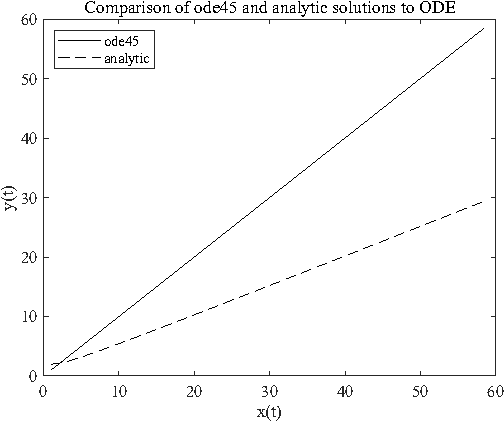
\includegraphics[width=\textwidth]{../ode_comp.pdf}
\end{figure}

\end{document}
